\chapter{Theoretical Background}
\label{chap:theory}

This chapter establishes the theoretical foundations necessary for understanding gravitational microlensing and the machine learning techniques applied in this work. We begin with the general relativistic basis of gravitational lensing (\cref{sec:grav_lensing}), then describe the characteristic features of microlensing light curves (\cref{sec:light_curves}), discuss observational considerations (\cref{sec:observations}), and finally introduce the machine learning methodology (\cref{sec:ml_methods}).

%%%%%%%%%%%%%%%%%%%%%%%%%%%%%%%%%%%%%%%%%%%%%%%%%%%%%%%%%%%%%
\section{Gravitational Lensing}
\label{sec:grav_lensing}

The phenomenon of light deflection by massive objects represents one of the most striking predictions of Einstein's general theory of relativity. In 1915, Einstein showed that spacetime curvature caused by mass would bend the path of light rays passing nearby. This prediction was famously confirmed during the solar eclipse of 1919, when Arthur Eddington observed the apparent displacement of stars near the Sun's limb \citep{Dyson1920}. The measured deflection of approximately $1.75$ arcseconds agreed closely with Einstein's prediction and was twice the value expected from Newtonian gravity. This result, widely publicized in the press, made Einstein a household name and inaugurated the study of gravitational lensing.

While early observations focused on strong lensing effects by galaxies—producing multiple resolved images and dramatic Einstein rings—gravitational microlensing operates on much smaller angular scales. Rather than resolving separate images, microlensing by individual stars manifests as temporary brightness variations in background sources. The image separations are of order milli-arcseconds, too small to be resolved with current instruments; instead, microlensing is detected through time-varying brightness changes.

In this section, we develop the mathematical framework for gravitational lensing, beginning with the general relativistic foundation (\cref{sec:gr_foundation}), deriving the fundamental lens equation (\cref{sec:lens_equation}), and explaining why stellar-mass lenses constitute the microlensing regime (\cref{sec:microlensing_basics}).

\subsection{General Relativistic Foundation}
\label{sec:gr_foundation}

The deflection of light by gravitational fields emerges naturally from Einstein's field equations. In the weak field limit, appropriate for most astrophysical lensing scenarios, we can treat the problem using the Schwarzschild metric with small perturbations. General relativity predicts that light rays follow geodesics in curved spacetime. For a non-rotating, spherically symmetric mass $M$, the line element is given by the Schwarzschild metric. In the weak-field limit where $2GM/(c^2 r) \ll 1$, one can treat the Newtonian potential $\Phi(r) = -GM/r$ as a perturbation to flat spacetime.

Consider a light ray passing at impact parameter $b$ from a point mass $M$. The spacetime curvature induces a deflection of the light path by an angle given by
\begin{equation}
  \alpha = \frac{4 G M}{c^2 b},
  \label{eq:deflection}
\end{equation}
where $G$ is the gravitational constant and $c$ is the speed of light. This deflection angle is twice the value predicted by a purely Newtonian treatment, increases with the mass of the lens, and decreases with the impact parameter, reflecting the inverse relationship between gravitational influence and distance.

The derivation can be made explicit by expanding the Schwarzschild metric to first order in $GM/(c^2 r)$ and computing the change in the transverse component of the photon's momentum. Alternatively, one may use Fermat's principle with an effective refractive index $n(r) \approx 1 - 2\Phi(r)/c^2$ to recover the same result. This provides an illuminating analogy: light bends in a gravitational field much as it would in a medium with spatially varying refractive index, with light rays preferentially following paths through regions of stronger gravitational potential.

For our purposes, the key insight is that \cref{eq:deflection} depends only on the total mass and geometric configuration, not on the specific composition or structure of the lens. This universality makes gravitational lensing a powerful probe of dark matter and compact objects, as the lensing signal directly traces the mass distribution regardless of luminosity.

\subsection{The Lens Equation}
\label{sec:lens_equation}

To formalize the relationship between source position and observed image position, we construct the lens equation in the thin lens approximation. We define the angular position of the source in the absence of lensing as $\boldsymbol{\beta}$, measured from the optical axis connecting the observer and lens. The observed angular position of the image is $\boldsymbol{\theta}$, also measured from this axis. Gravitational lensing describes how a lens mass at position $\boldsymbol{\theta}$ maps rays from a source at position $\boldsymbol{\beta}$ to images on the observer's sky.

The lens equation relates these quantities through the deflection angle. In the simplest case of an axisymmetric point-mass lens, the two angular variables become scalars $\beta$ and $\theta$ measured from the optical axis. The lens equation can then be written as
\begin{equation}
  \beta = \theta - \frac{\theta_E^2}{\theta},
  \label{eq:lens_eq}
\end{equation}
where $\theta_E$ is the Einstein radius. This equation is obtained by projecting the geometry of the lensing system and relating the true source position to the observed image position through the deflection angle.

When the source lies directly behind the lens ($\beta=0$), the lens equation predicts a ring of images of angular radius $\theta_E$, known as an Einstein ring. The angular Einstein radius depends on the lens mass and the distances between observer, lens, and source:
\begin{equation}
  \theta_E = \sqrt{\frac{4 G M}{c^2} \frac{D_{\mathrm{ls}}}{D_{\mathrm{l}} D_{\mathrm{s}}}},
  \label{eq:einstein_ang}
\end{equation}
where $D_{\mathrm{l}}$ is the angular-diameter distance from observer to lens, $D_{\mathrm{s}}$ is the distance from observer to source, and $D_{\mathrm{ls}}$ is the distance from lens to source. In physical units the Einstein radius in the source plane is
\begin{equation}
  R_E = \sqrt{\frac{4 G M}{c^2} \frac{D_{\mathrm{l}} D_{\mathrm{ls}}}{D_{\mathrm{s}}}}.
  \label{eq:einstein_phys}
\end{equation}

The Einstein radius represents the characteristic angular scale of the lensing effect: it separates two regimes of lensing behavior. For source positions $\beta \ll \theta_E$, the lens creates significant magnification and distortion. For $\beta \gg \theta_E$, lensing effects become negligible. For a stellar-mass lens in the Galactic bulge, $\theta_E$ is of order microarcseconds, so the two images lie too close to be resolved individually. Nevertheless, the total magnification of the source depends sensitively on the alignment encoded in \cref{eq:lens_eq}; this sensitivity underlies the microlensing phenomena discussed below.

\begin{figure}[htbp]
    \centering
    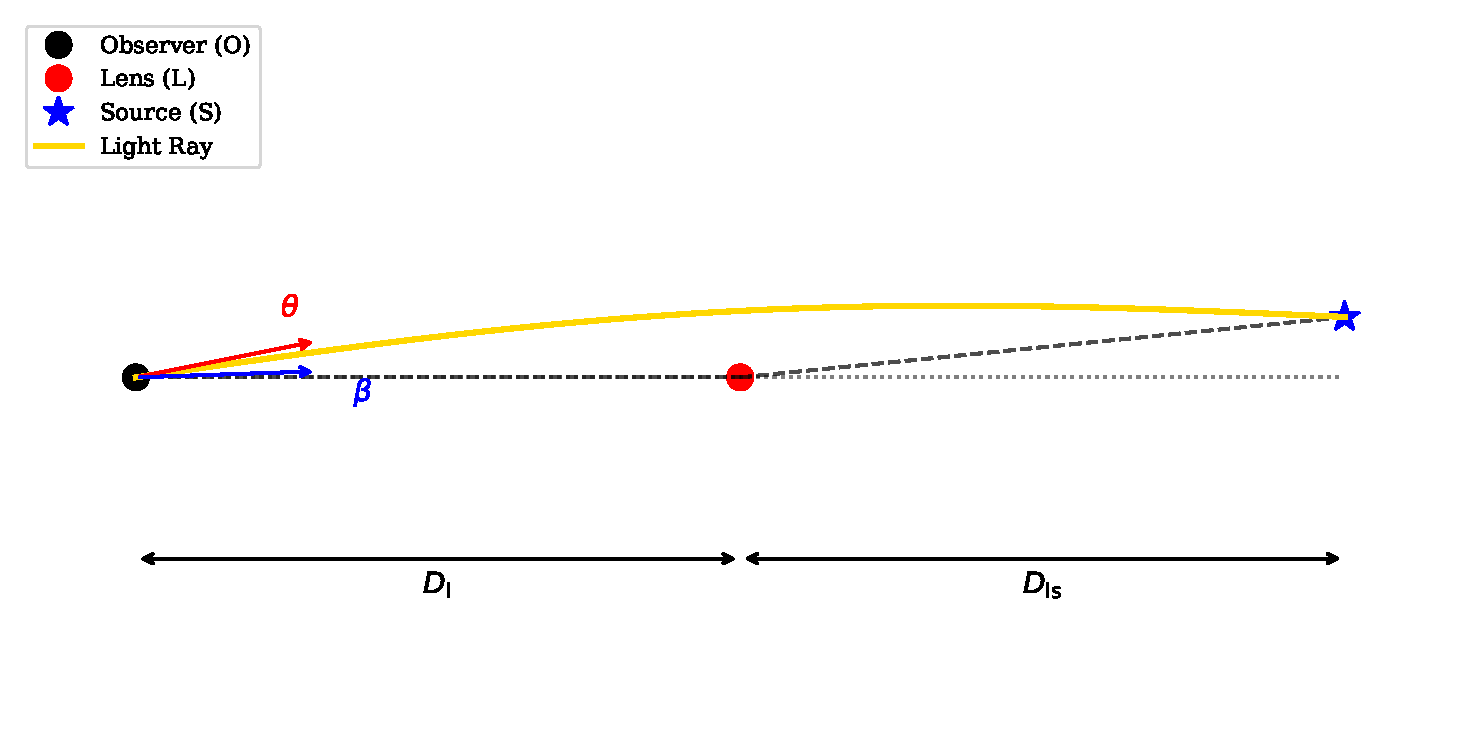
\includegraphics[width=0.85\textwidth]{figures/fig_lens_geometry.pdf}
    \caption[Gravitational lens geometry.]{Schematic diagram of gravitational lens geometry. The observer (O), lens (L), and source (S) are shown with their respective angular diameter distances ($D_\mathrm{l}$, $D_\mathrm{s}$, $D_\mathrm{ls}$). The true source position is $\beta$, the image position is $\theta$, and the light ray is deflected by angle $\alpha$. The Einstein radius $\theta_E$ represents the characteristic angular scale of the lensing effect.}
    \label{fig:lens_geometry}
\end{figure}

\subsection{Gravitational Microlensing}
\label{sec:microlensing_basics}

When the angular Einstein radius is micro-arcsecond, individual lensed images cannot be resolved with current instruments. Instead, observers detect microlensing through the time-dependent magnification of the source flux as the lens–source alignment evolves. The microlensing regime thus differs from strong lensing: no multiple images are seen, and the light curve is symmetric in time for a single lens. Because the image separations are ${\sim}$milli-arcseconds, only the combined flux matters.

Microlensing events occur when a foreground star (or planetary system) passes close to the line of sight to a background star, producing a characteristic brightening and fading. The Einstein radius sets both the angular scale and the time scale of the event; typical Galactic events have Einstein crossing times of days to months, depending on the lens mass and relative motion.

Microlensing is achromatic for a point source because the lensing magnification is wavelength-independent, although finite-source effects can introduce chromaticity at very high magnifications. The characteristic timescale, known as the Einstein crossing time $t_E$, represents the time for the source to traverse an Einstein radius due to the relative proper motion between lens and source. Section~\ref{sec:light_curves} develops the formalism needed to model microlensing light curves and to interpret their parameters.

%%%%%%%%%%%%%%%%%%%%%%%%%%%%%%%%%%%%%%%%%%%%%%%%%%%%%%%%%%%%%
\section{Microlensing Light Curves}
\label{sec:light_curves}

The light curve of a microlensing event encodes the geometry and kinematics of the lens–source system. In the simplest case of a point source lensed by a single point mass, the flux increases smoothly to a maximum and then declines symmetrically. More complex lenses (e.g., binaries) or finite source sizes introduce caustics, asymmetries and multiple peaks. In this section we derive the standard point-source point-lens (PSPL) magnification formula (\cref{sec:pspl}), define key parameters, outline the effects of binary lenses (\cref{sec:binary_lensing}), and summarize finite-source effects (\cref{sec:finite_source}).

\subsection{Point-Source Point-Lens (PSPL) Model}
\label{sec:pspl}

For a point source lensed by a single mass, the total magnification $A$ of the unresolved images can be expressed in terms of the dimensionless separation $u$ (in units of $\theta_E$) between the lens and the source. A derivation from the Jacobian of the lens mapping yields
\begin{equation}
  A(u) = \frac{u^2 + 2}{u \sqrt{u^2 + 4}},
  \label{eq:pspl_mag}
\end{equation}
where $u = |\boldsymbol{\beta}|/\theta_E$ is the source–lens separation in units of the Einstein radius. This formula shows that magnification increases as $u$ decreases, becoming formally infinite when the source and lens are perfectly aligned ($u=0$). In practice, finite source size limits the maximum magnification, a point we return to in \cref{sec:finite_source}.

If the lens moves with constant velocity relative to the source, the separation $u(t)$ varies as
\begin{equation}
  u(t) = \sqrt{u_0^2 + \left(\frac{t - t_0}{t_E}\right)^2},
  \label{eq:u_of_t}
\end{equation}
where $u_0$ is the minimum impact parameter (closest approach in units of $\theta_E$), $t_0$ is the time of closest approach, and $t_E$ is the Einstein crossing time. The Einstein time represents the characteristic duration of the event and is defined as
\begin{equation}
  t_E = \frac{R_E}{v_\perp},
  \label{eq:einstein_time}
\end{equation}
where $v_\perp$ is the transverse velocity of the lens relative to the source. Combining \cref{eq:pspl_mag} and \cref{eq:u_of_t} gives the PSPL light curve as a function of time.

The observed flux in a microlensing event is
\begin{equation}
  F(t) = F_{\mathrm{base}} + F_{\mathrm{source}} \left[A(u(t)) - 1\right],
  \label{eq:flux}
\end{equation}
where $F_{\mathrm{base}}$ is the baseline flux (including any blended light from unresolved stars) and $F_{\mathrm{source}}$ is the unlensed flux of the source. This equation accounts for the fact that only the source is magnified, not any blended stars in the same resolution element.

The PSPL model is characterized by three physical parameters: $u_0$, $t_0$, and $t_E$. Events with small $u_0$ (close alignment) produce high-magnification light curves with sharp peaks, while events with large $u_0$ produce broad, low-amplitude variations. The Einstein time $t_E$ sets the overall duration of the event, with shorter times indicating either lower-mass lenses or higher relative velocities. For typical Galactic bulge events, $t_E$ ranges from roughly 10 to 150 days.

\begin{figure}[htbp]
    \centering
    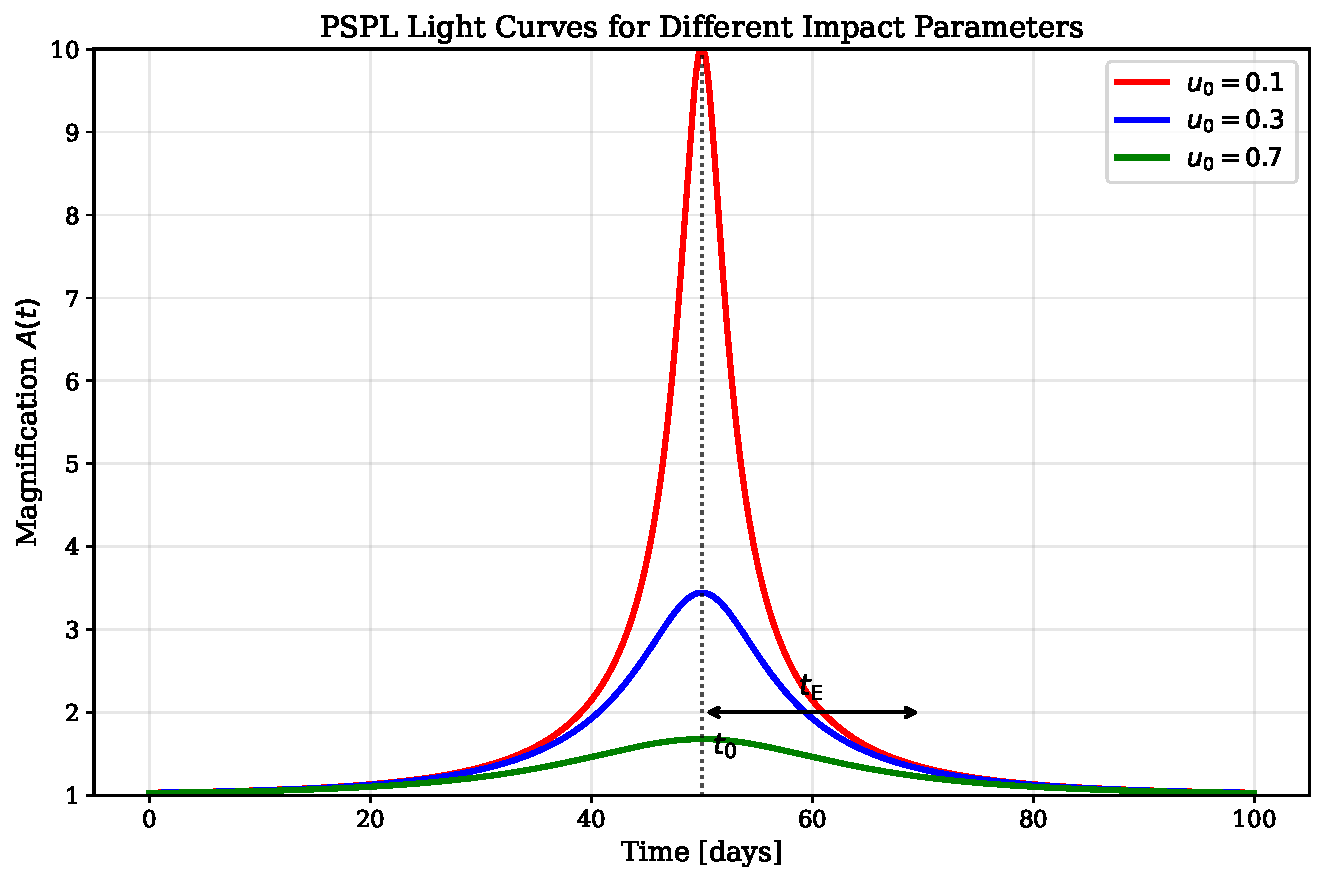
\includegraphics[width=0.9\textwidth]{figures/fig_pspl_lightcurve.pdf}
    \caption[PSPL light curves for different impact parameters.]{Point Source Point Lens (PSPL) light curves for three different impact parameters: $u_0 = 0.1$ (high magnification, red), $u_0 = 0.3$ (moderate magnification, blue), and $u_0 = 0.7$ (low magnification, green). The time of closest approach $t_0$ and Einstein crossing time $t_E$ are indicated. The symmetric shape and smooth profiles are characteristic of single-lens events.}
    \label{fig:pspl_lightcurve}
\end{figure}

\begin{figure}[htbp]
    \centering
    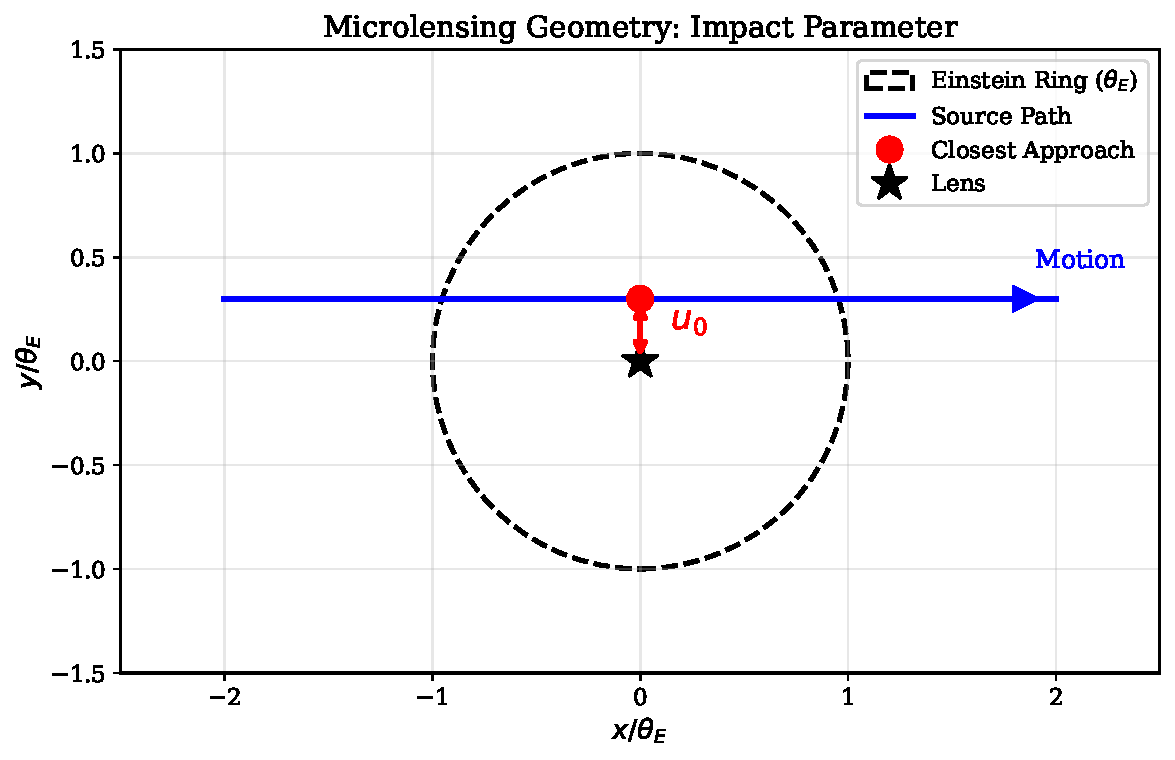
\includegraphics[width=0.75\textwidth]{figures/fig_impact_parameter.pdf}
    \caption[Microlensing geometry showing impact parameter.]{Geometric representation of the impact parameter $u_0$ in microlensing. The source (blue trajectory) moves with respect to the lens (black star at origin). The Einstein ring (dashed circle) has radius $\theta_E$. The minimum separation between the source path and the lens defines the impact parameter $u_0$, measured in units of the Einstein radius. Smaller impact parameters result in higher magnification events.}
    \label{fig:impact_parameter}
\end{figure}

\subsection{Binary Lenses}
\label{sec:binary_lensing}

When the lens consists of two masses—such as a star with a planetary companion—the lensing geometry becomes significantly more complex. Binary lenses introduce additional parameters: the projected separation $s$ (in units of $\theta_E$), the mass ratio $q = M_2/M_1$, and the angle $\alpha$ defining the source trajectory relative to the binary axis. For binary separations near $s \sim 1$, the caustic structure creates regions where the magnification is formally infinite (for point sources) or extremely large (for finite sources).

The magnification for a binary lens cannot be written in closed form like \cref{eq:pspl_mag}. Instead, it must be computed either by solving a fifth-order complex polynomial at each time step or by using ray-tracing techniques that simulate the paths of many light rays through the lens system. The resulting light curves exhibit characteristic features that distinguish them from PSPL events:

\begin{itemize}
  \item \textbf{Caustic crossings:} When the source crosses a caustic, the light curve shows sharp spikes or bumps lasting a fraction of $t_E$. The spike shape depends on the source size and the crossing speed.
  \item \textbf{Asymmetric profiles:} Binary light curves are typically asymmetric, with the rise and fall times differing depending on the source trajectory relative to the caustic structure.
  \item \textbf{Multiple peaks:} Depending on the geometry, a source may cross multiple caustic features, producing light curves with two or more distinct peaks.
  \item \textbf{Longer duration anomalies:} Even without caustic crossings, the perturbation from the companion can create extended deviations from the PSPL profile lasting days to weeks.
\end{itemize}

Planetary companions with mass ratios $q \sim 10^{-3}$ to $10^{-4}$ produce caustics that are small compared to the primary Einstein radius. The probability of detecting such planets depends on the survey cadence: high-frequency observations (multiple times per night) are essential to capture short-duration caustic crossings that might otherwise be missed. The complexity of binary lens modeling motivates the machine learning approach developed in this thesis, as traditional fitting methods become computationally prohibitive when analyzing thousands of events in real time.

\begin{figure}[htbp]
    \centering
    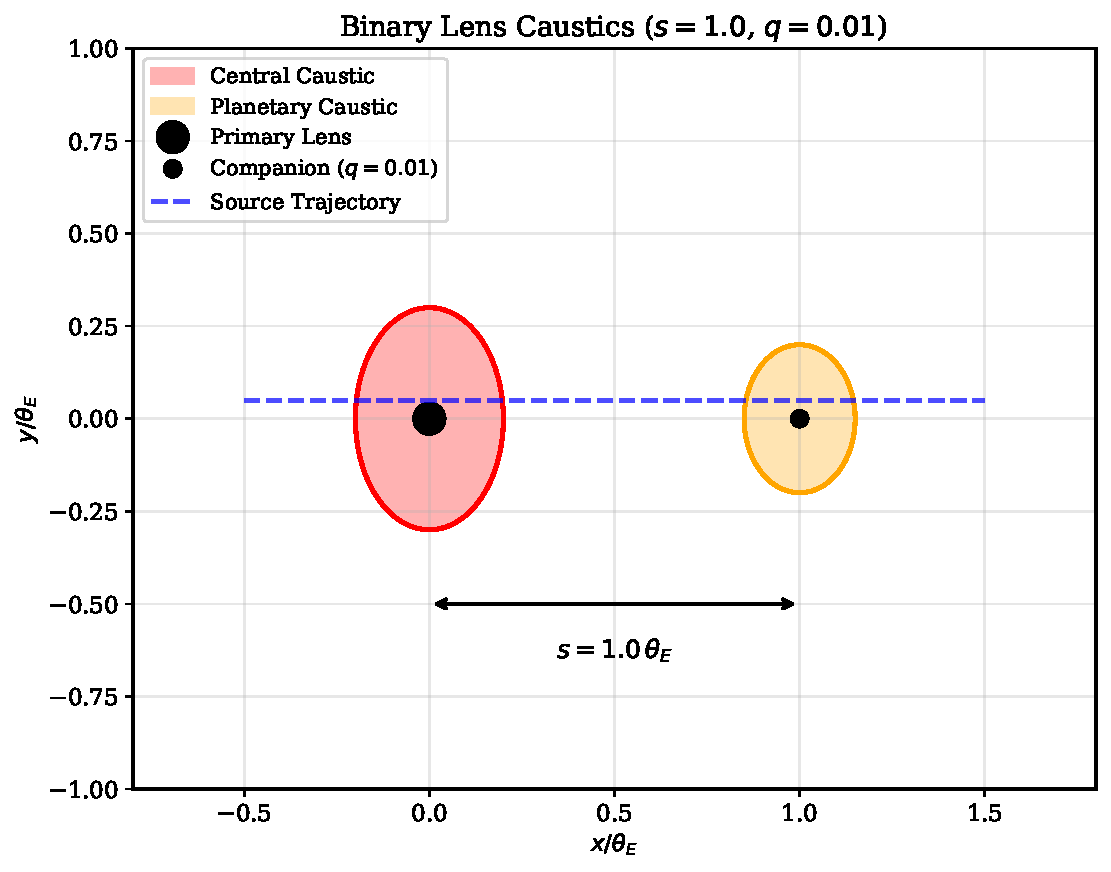
\includegraphics[width=0.8\textwidth]{figures/fig_binary_caustics.pdf}
    \caption[Binary lens caustic structure.]{Illustration of binary lens caustics for a system with separation $s = 1.0$ and mass ratio $q = 0.01$ (representative of a planetary companion). The red central caustic and orange planetary caustic represent regions where magnification becomes extremely large. The two black dots indicate the lens positions (primary at origin, companion at $x = 1.0\,\theta_E$). A source trajectory (blue dashed line) crossing or passing near these caustics produces characteristic deviations from PSPL behavior. The caustic topology depends sensitively on the separation $s$ and mass ratio $q$.}
    \label{fig:binary_caustics}
\end{figure}

\begin{figure}[htbp]
    \centering
    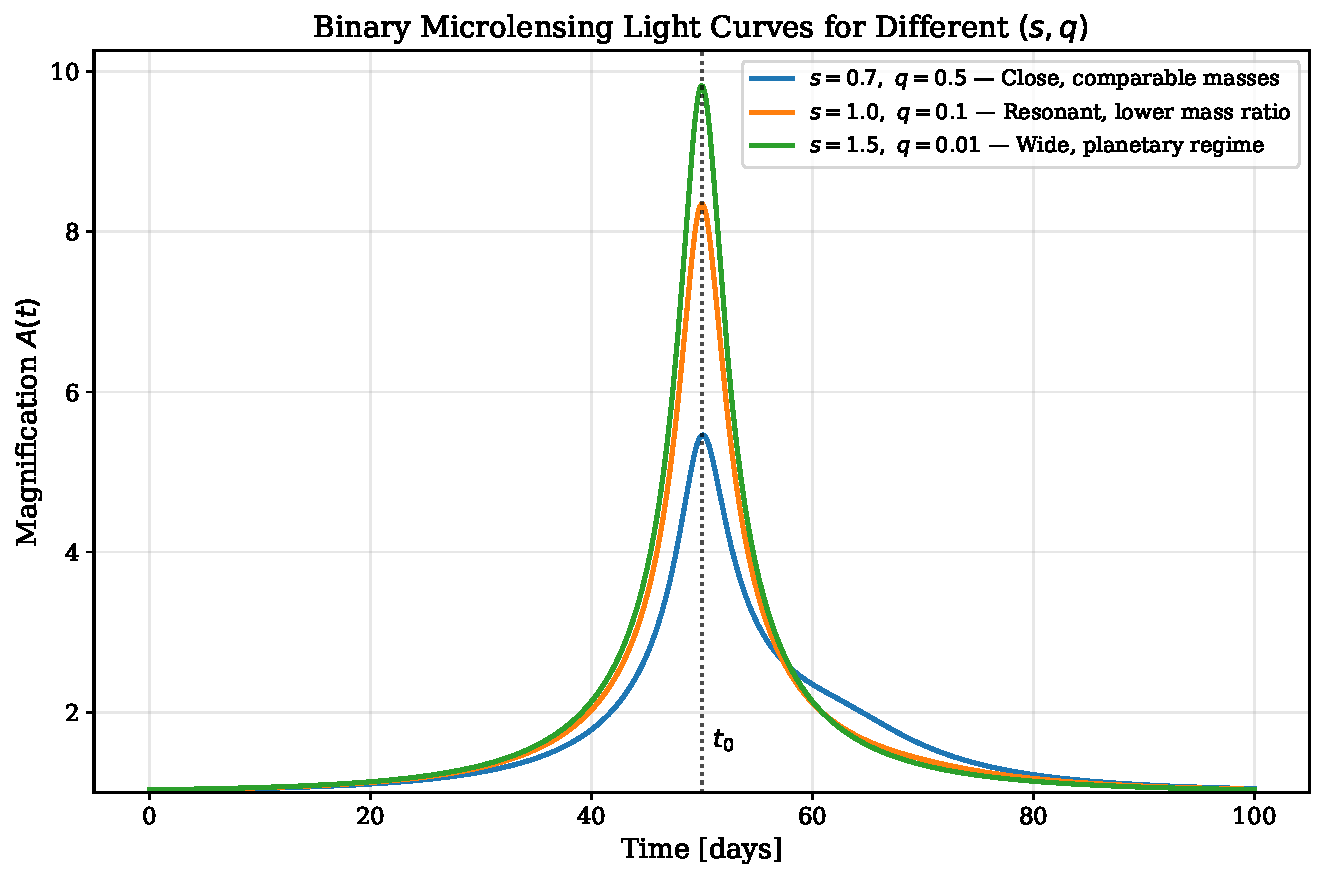
\includegraphics[width=0.9\textwidth]{figures/fig_binary_lightcurves.pdf}
    \caption[Examples of binary microlensing light curves.]{Binary microlensing light curves showing diverse morphologies depending on source trajectory and binary parameters. Top: Caustic crossing event with sharp spike. Middle: Near-caustic event with asymmetric perturbation. Bottom: Resonant caustic event with multiple peaks. These features distinguish binary events from the smooth, symmetric PSPL profile and motivate the use of machine learning for automated classification.}
    \label{fig:binary_lightcurves}
\end{figure}

\subsection{Finite Source Effects}
\label{sec:finite_source}

The point-source approximation breaks down when $u$ becomes comparable to the source radius $\rho$ (in units of $\theta_E$). For a source of angular radius $\theta_*$, the dimensionless source size is $\rho = \theta_*/\theta_E$. Typical main-sequence stars in the Galactic bulge have $\rho \sim 10^{-3}$ to $10^{-2}$, becoming important only for high-magnification events with $u_0 \lesssim \rho$.

Finite source size modifies the light curve in two ways. First, it limits the maximum magnification: instead of diverging as $u \to 0$, the magnification saturates at a finite value determined by limb darkening and the source profile. Second, during caustic crossings in binary events, finite source size smooths the sharp features predicted for point sources, broadening the spikes into rounded peaks with characteristic widths determined by $\rho$ and the crossing speed.

Finite source effects are crucial for determining lens masses through measurements of the Einstein radius crossing time and the microlensing parallax. However, for the machine learning classification task in this thesis, we focus primarily on distinguishing the overall morphological differences between PSPL and binary light curves rather than on precise parameter estimation that requires accounting for finite source size.

%%%%%%%%%%%%%%%%%%%%%%%%%%%%%%%%%%%%%%%%%%%%%%%%%%%%%%%%%%%%%
\section{Observational Strategies}
\label{sec:observations}

Detecting and characterizing microlensing events requires sustained, high-cadence monitoring of millions of stars in crowded fields. Modern surveys employ difference imaging analysis (DIA) to overcome the challenges of crowding and varying seeing conditions. In this section we describe the observational techniques used by current surveys (\cref{sec:surveys}), photometric challenges related to blending and baseline flux (\cref{sec:photometric_challenges}), and the requirements for detecting planetary signals (\cref{sec:obs_challenges}).

\subsection{Survey Overview}
\label{sec:surveys}

The two major ground-based microlensing surveys, OGLE (Optical Gravitational Lensing Experiment) and MOA (Microlensing Observations in Astrophysics), have been monitoring the Galactic bulge for over two decades. OGLE operates a 1.3-m telescope at Las Campanas Observatory in Chile and monitors approximately 200 million stars across roughly 600 square degrees. The OGLE Early Warning System issues real-time alerts for ongoing events with high magnification, enabling follow-up observations by other groups. MOA uses a 1.8-m telescope at Mount John Observatory in New Zealand and monitors approximately 17 square degrees of the bulge with sampling rates up to six times per night.

Future space-based missions will revolutionize microlensing surveys. The Nancy Grace Roman Space Telescope, scheduled for launch in the mid-2020s, will conduct a dedicated microlensing survey monitoring the Galactic bulge from space, free from weather interruptions and atmospheric seeing effects. Roman's wide-field infrared camera will observe 2.8 square degrees with unprecedented photometric precision, detecting thousands of microlensing events per year and enabling the detection of planets down to Mars mass. The Vera C. Rubin Observatory's Legacy Survey of Space and Time (LSST) will also contribute to microlensing science through its deep, wide-area, time-domain survey, though its observing strategy is optimized for transient detection rather than continuous monitoring.

\subsection{Photometric Challenges}
\label{sec:photometric_challenges}

Difference imaging analysis (DIA) subtracts a high-quality reference image from each new observation to isolate flux variations. This technique is essential in crowded fields where traditional aperture photometry fails due to overlapping stellar point spread functions (PSFs). However, DIA introduces its own challenges. The baseline flux (unmagnified flux) of a source is not measured directly in the difference image and must be estimated separately. If the baseline flux is mis-estimated, the inferred magnification curve can be mis-normalized, leading to degeneracies in the fit. High-magnification events are less affected because even a small fractional error in baseline flux produces a noticeable deviation in the light curve.

Blending remains a significant source of systematic error. Blending occurs when multiple stars fall within the same PSF, causing the measured flux to include light from both the lensed source and unresolved neighbors. Imperfect deblending increases the measured background, causing a magnitude bias near the detection threshold; faint stars can disappear within the combined PSF of brighter neighbors; and centroid motions induced by blending can bias the flux measurement. If blending is neglected in modeling, the impact parameter $u_0$ tends to be overestimated and the Einstein time $t_E$ underestimated, biasing optical depth estimates. Even bright stars are often blended and require careful modeling.

Extinction and reddening by interstellar dust further modify observed colors and must be accounted for when comparing different fields. The complex dust distribution toward the Galactic bulge creates significant variations in extinction across the field, requiring color-dependent corrections that can introduce additional systematic uncertainties.

\subsection{Observational Challenges}
\label{sec:obs_challenges}

Monitoring millions of stars night after night poses logistical and technical challenges. Crowded fields demand high image quality and consistent PSF across the field; variable seeing and weather conditions introduce systematic errors that complicate DIA. Detection thresholds vary across the field because the background is dominated by merged stellar wings, and changes in seeing can overwhelm deblending algorithms.

Real-time event detection and follow-up are essential for capturing short perturbations caused by planets. High-magnification events are of particular interest because they have high planet detection efficiencies. Automated anomaly detectors trigger increased sampling when deviations from the PSPL model are seen. A high-cadence strategy may employ survey observations every day, follow-up observations every $\sim$90 minutes near peak, and anomaly monitoring every few minutes when an unexpected deviation occurs. Such multi-tiered cadence maximizes the probability of detecting short-lived planetary signals.

Weather interruptions, moonlight and seasonal visibility limit the temporal coverage from a single site, necessitating networks of telescopes around the globe. Robotic networks and automated analysis pipelines (e.g., OGLE's Early Warning System and MOA's real-time DIA) have become standard tools for coordinating follow-up observations. The development of machine learning classifiers that can rapidly identify anomalous events in real time represents a natural extension of these automated systems, enabling more efficient allocation of follow-up resources.

%%%%%%%%%%%%%%%%%%%%%%%%%%%%%%%%%%%%%%%%%%%%%%%%%%%%%%%%%%%%%
\section{Machine Learning for Time Series}
\label{sec:ml_methods}

Traditional microlensing analyses fit parametric models to each event, a process that can be computationally intensive and requires good initial guesses for non-linear parameters. Machine learning offers an alternative approach: by training on simulated and observed light curves, an ML model can learn to recognize microlensing events and infer parameters quickly. For large surveys expecting thousands of events per year, automatic classification and real-time parameter estimation become invaluable.

Machine learning circumvents computational bottlenecks by reframing the problem as pattern recognition. Rather than searching parameter space for each new observation, a neural network learns to recognize characteristic patterns in light curves that correlate with specific physical scenarios. After an initial training phase—which may be computationally expensive—inference on new light curves becomes nearly instantaneous, requiring only a forward pass through the network. This speed advantage is crucial for real-time classification systems that must process hundreds of ongoing events to prioritize follow-up observations.

What makes microlensing particularly amenable to machine learning approaches? Several factors contribute: first, the underlying physical model is well-understood and deterministic, allowing generation of essentially unlimited training data through simulation. Second, light curves exhibit characteristic morphologies—smooth symmetric rises for PSPL events, sharp caustic crossing spikes for binaries—that should be recognizable to pattern-matching algorithms. Third, the photometric time series is relatively low-dimensional compared to images, making network architectures tractable without requiring massive computational resources.

In this section we outline why ML is suitable for microlensing time series, introduce convolutional neural networks (CNNs) as the architecture used in this thesis (\cref{sec:cnn_fundamentals}), describe their application to one-dimensional time series data (\cref{sec:cnn_1d}), and explain the training and validation strategies we employ (\cref{sec:training_strategies}).

\subsection{Convolutional Neural Networks}
\label{sec:cnn_fundamentals}

Convolutional neural networks (CNNs) have emerged as the dominant architecture for learning from data with spatial or temporal structure. Unlike fully connected neural networks, where every neuron connects to every neuron in adjacent layers, CNNs exploit local structure through convolutional layers that apply learned filters across the input. This design reflects two key principles: local patterns matter (nearby data points are more related than distant ones), and the same patterns can appear at different positions (translation invariance).

A typical CNN architecture consists of several key building blocks:

\begin{itemize}
  \item \textbf{Convolutional Layers:} This is the core component. A convolutional layer uses a set of small, learnable filters (kernels) that slide across the input data, performing dot products at each position. Each kernel detects a specific local feature—such as an edge in an image, or a sharp spike in a time series. The key insight is \textbf{parameter sharing}: the same kernel is used across the entire input, allowing the network to detect that feature regardless of where it appears. For a one-dimensional input $\mathbf{x}$ and kernel weights $\mathbf{w}$, the output at position $i$ is
  \begin{equation}
    y[i] = \sum_{k=0}^{K-1} w[k] \cdot x[i+k] + b,
    \label{eq:1d_convolution}
  \end{equation}
  where $K$ is the kernel size and $b$ is a bias term. Multiple kernels are applied in parallel, each learning to detect different features.
  
  \item \textbf{Activation Functions:} After each convolution, the output is passed through a non-linear activation function, most commonly the Rectified Linear Unit (ReLU), defined as $f(x) = \max(0, x)$. This non-linearity allows the network to learn complex, non-trivial patterns. ReLU effectively zeros out negative activations while passing positive values unchanged, creating sparse representations where only a subset of neurons activate for any given input.
  
  \item \textbf{Pooling Layers:} These layers reduce dimensionality while retaining important features. Max pooling selects the maximum value within each local window, effectively downsampling the representation. Pooling provides translation invariance (small shifts in input don't dramatically change the pooled output), reduces computational cost in subsequent layers, and helps prevent overfitting by reducing the number of parameters.
  
  \item \textbf{Fully Connected Layers:} After several convolutional and pooling layers extract hierarchical features from the input, the features are flattened and fed into one or more fully connected layers, where each neuron is connected to all neurons in the previous layer. For classification tasks, the final layer typically uses a softmax activation to produce a probability distribution over classes.
\end{itemize}

The entire network is trained end-to-end using backpropagation, where gradients of a loss function with respect to all weights are computed and used to update parameters through optimization algorithms like Adam or stochastic gradient descent. This hierarchical structure allows a CNN to learn simple features (like sharpness or slopes) in early layers and then combine them into more complex, abstract features (like caustic-crossing anomalies) in deeper layers.

\subsection{1D CNNs for Time Series}
\label{sec:cnn_1d}

While CNNs were originally developed for two-dimensional image analysis, the same principles extend naturally to one-dimensional data like time series. A 1D CNN applies convolutions along the temporal axis, with kernels that learn to recognize patterns in sequences rather than spatial arrangements. For microlensing light curves, this architecture is particularly appropriate because the data is inherently sequential: flux measurements at different times constitute a one-dimensional signal.

Interpreting the kernel size as a temporal scale provides intuition for network design. For a CNN analyzing microlensing light curves with $\sim$100 observations spanning $\sim$100 days, a kernel of size 5 effectively examines 5-day windows, appropriate for detecting short-timescale planetary anomalies. Kernels of size 11 or 15 capture the overall shape of PSPL events. By stacking multiple convolutional layers with varying kernel sizes, the network builds a hierarchy of representations: early layers detect local features such as the symmetric rise and fall of a microlensing event or the sharper spikes produced by caustic crossings, while deeper layers combine these into higher-level patterns that span the entire light curve.

One advantage of 1D CNNs for irregularly sampled data is their flexibility with input representation. One-dimensional convolutions naturally handle irregular sampling if time bins are uniform after interpolation or binning. Rather than requiring evenly spaced time points, light curves can be preprocessed into regularly sampled representations. For most microlensing applications, simple interpolation to a fixed grid (e.g., 128 or 256 time bins spanning the event duration) provides a reasonable compromise between preserving information and maintaining tractable network architectures. The 1D CNN architecture requires fewer parameters than fully connected networks, reducing overfitting and computational cost.

The architecture used in this thesis employs several 1D convolution and pooling layers followed by dense layers to classify events and estimate parameters. Subsequent pooling layers aggregate local features, enabling the network to detect features irrespective of their exact timing, providing robustness to small temporal shifts and irregular sampling patterns.

\begin{figure}[htbp]
    \centering
    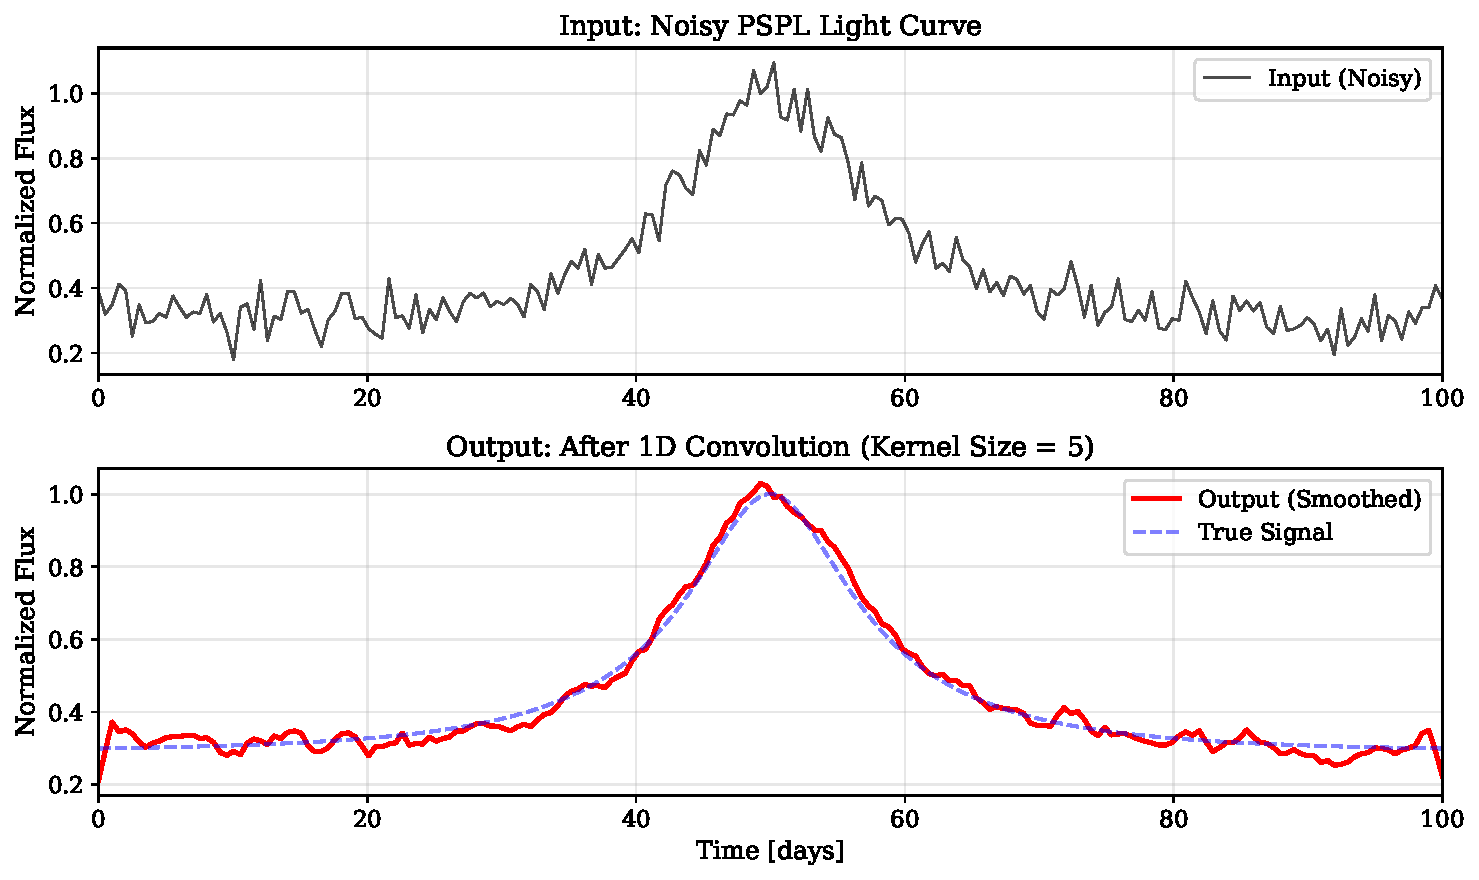
\includegraphics[width=0.95\textwidth]{figures/fig_convolution_example.pdf}
    \caption[Example of 1D convolution on a light curve.]{Demonstration of 1D convolution applied to a noisy PSPL light curve. Top panel: Input light curve with photometric noise (black). Bottom panel: Output after applying a 5-point smoothing kernel (red) compared to the true underlying signal (blue dashed). The convolution operation extracts local temporal features while reducing noise, illustrating how convolutional layers in a CNN can learn to recognize characteristic patterns in microlensing data.}
    \label{fig:convolution_example}
\end{figure}

\begin{figure}[htbp]
    \centering
    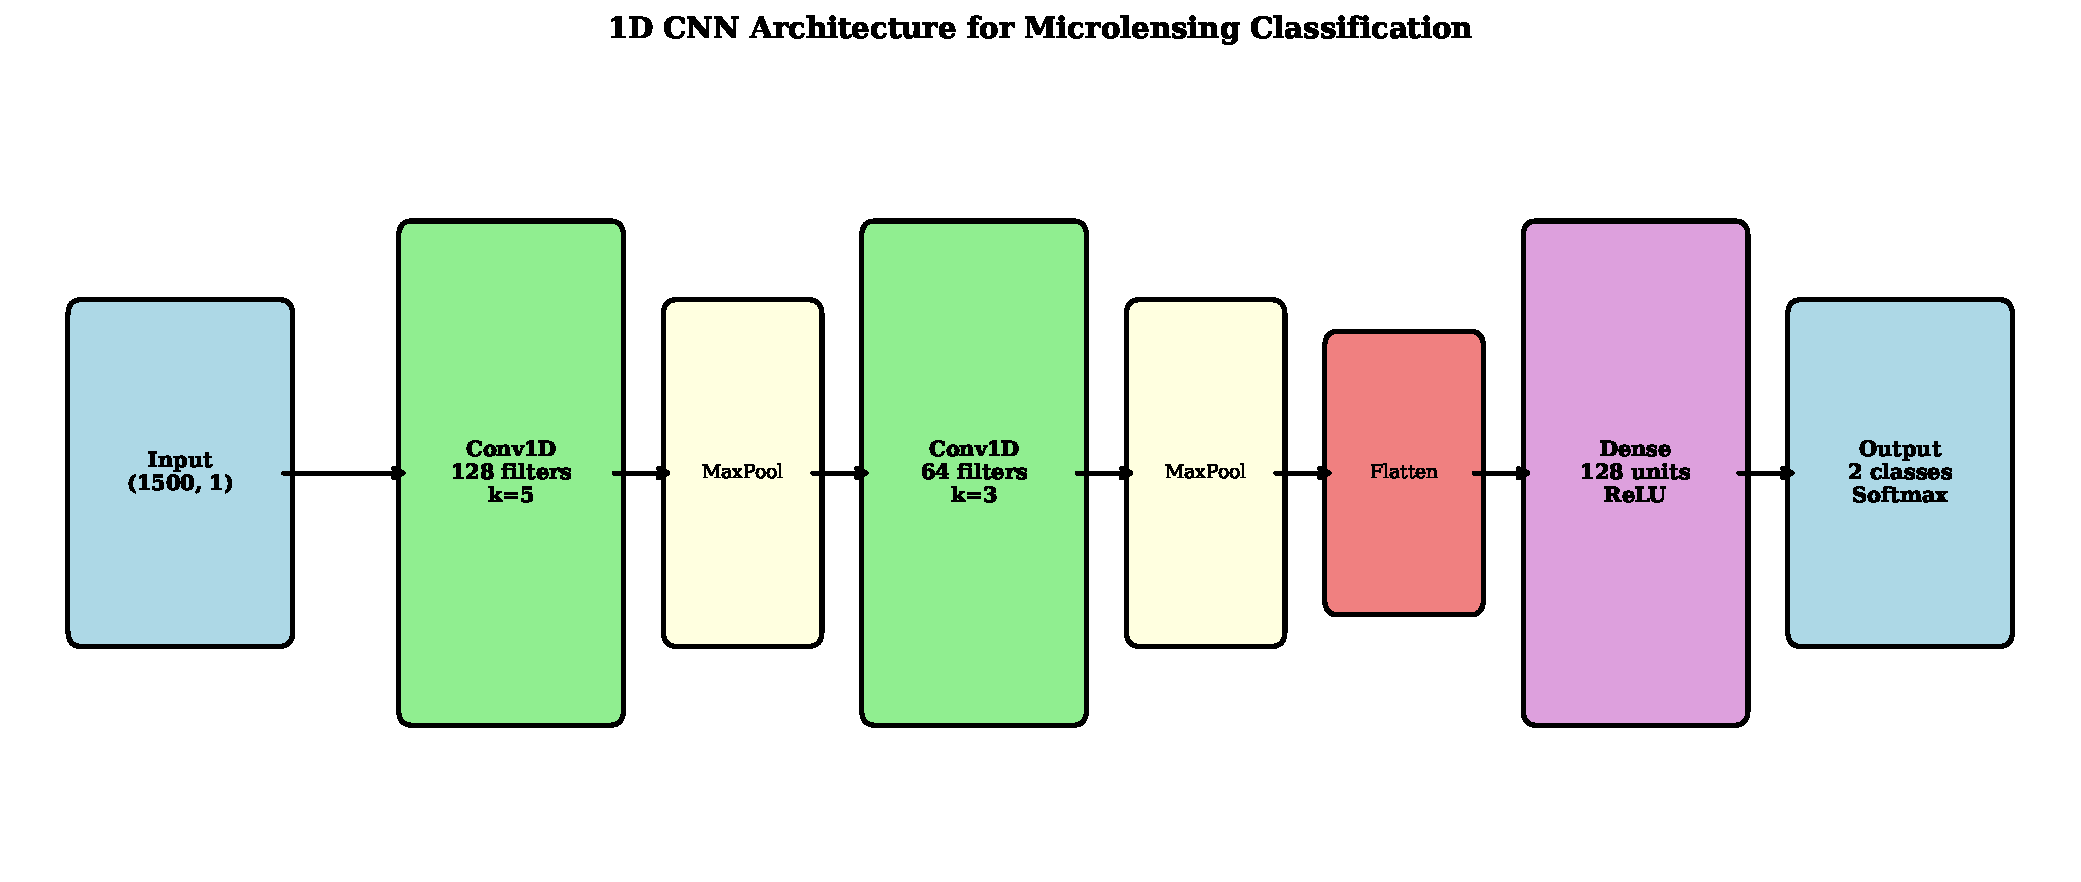
\includegraphics[width=\textwidth]{figures/fig_cnn_architecture.pdf}
    \caption[1D CNN architecture for microlensing classification.]{Schematic diagram of the 1D Convolutional Neural Network architecture used in this thesis. The input light curve (1500 timesteps) passes through alternating convolutional (Conv1D) and pooling layers that extract hierarchical features at different temporal scales. After feature extraction, the data is flattened and passed through fully connected (Dense) layers to produce the final binary classification (PSPL vs. Binary) using a softmax activation. Dropout layers (not shown) are applied after each convolutional layer to prevent overfitting.}
    \label{fig:cnn_architecture}
\end{figure}

\subsection{Training and Validation Strategies}
\label{sec:training_strategies}

Training a neural network for microlensing classification requires careful dataset partitioning, regularization to prevent overfitting, and appropriate evaluation metrics. Successful machine learning requires careful handling of the training data and model capacity.

The available dataset is typically divided into three subsets: a training set to fit the model (typically 70–80\%), a validation set to tune hyperparameters and monitor overfitting (10–15\%), and a test set to provide an unbiased estimate of performance on unseen data (10–15\%). Each partition should contain balanced representations of both PSPL and binary events to ensure the model learns from diverse examples.

To prevent overfitting, regularization techniques such as early stopping and dropout are employed. Early stopping monitors the validation loss during training and halts training when the loss ceases to decrease, thus avoiding the deterioration of generalization performance. Dropout randomly disables a fraction of neurons during each training step (typically 20–50\%), preventing them from co-adapting and reducing overfitting.

For classification tasks, the cross-entropy loss function
\begin{equation}
  \mathcal{L} = -\sum_{c=1}^{C} y_c \log(\hat{y}_c)
  \label{eq:cross_entropy}
\end{equation}
is commonly used, where $y_c$ is the true class label (one-hot encoded) and $\hat{y}_c$ is the predicted probability for class $c$. Evaluation metrics such as accuracy, precision and recall quantify the performance of the classifier on the test set.

For classification, we use standard metrics: \textbf{accuracy} (overall correct classification rate), \textbf{precision} (fraction of predicted binaries that are truly binary), and \textbf{recall} (fraction of true binaries correctly identified). For imbalanced datasets where one class is rare, precision and recall are often more informative than simple accuracy. The $F_1$ score, the harmonic mean of precision and recall, provides a single metric balancing both concerns. For regression tasks such as predicting event parameters, metrics like mean absolute error or root mean square error are used.

When data are limited, cross-validation can be employed: the dataset is split into $k$ folds, with each fold serving as the test set once while the others form the training set. The results are averaged to obtain a robust estimate of performance. However, for large simulated datasets with millions of examples, a simple train–validation–test split typically suffices.

In this thesis we adopt a train–validation–test split, apply dropout and early stopping, and use cross-entropy loss to train a 1D CNN that classifies light curves and estimates microlensing parameters. The model is trained using the Adam optimizer with appropriate learning rates and batch sizes, with hyperparameters tuned based on validation set performance. For operational deployment, we focus on high-confidence predictions where the model's softmax probability exceeds a threshold (e.g., 0.8), ensuring reliable event classification for follow-up triggering decisions.